\documentclass[tikz,border=10pt]{standalone}
\usepackage{tikz}
\usetikzlibrary{shapes.geometric,arrows.meta,positioning,fit,backgrounds,calc}

\begin{document}
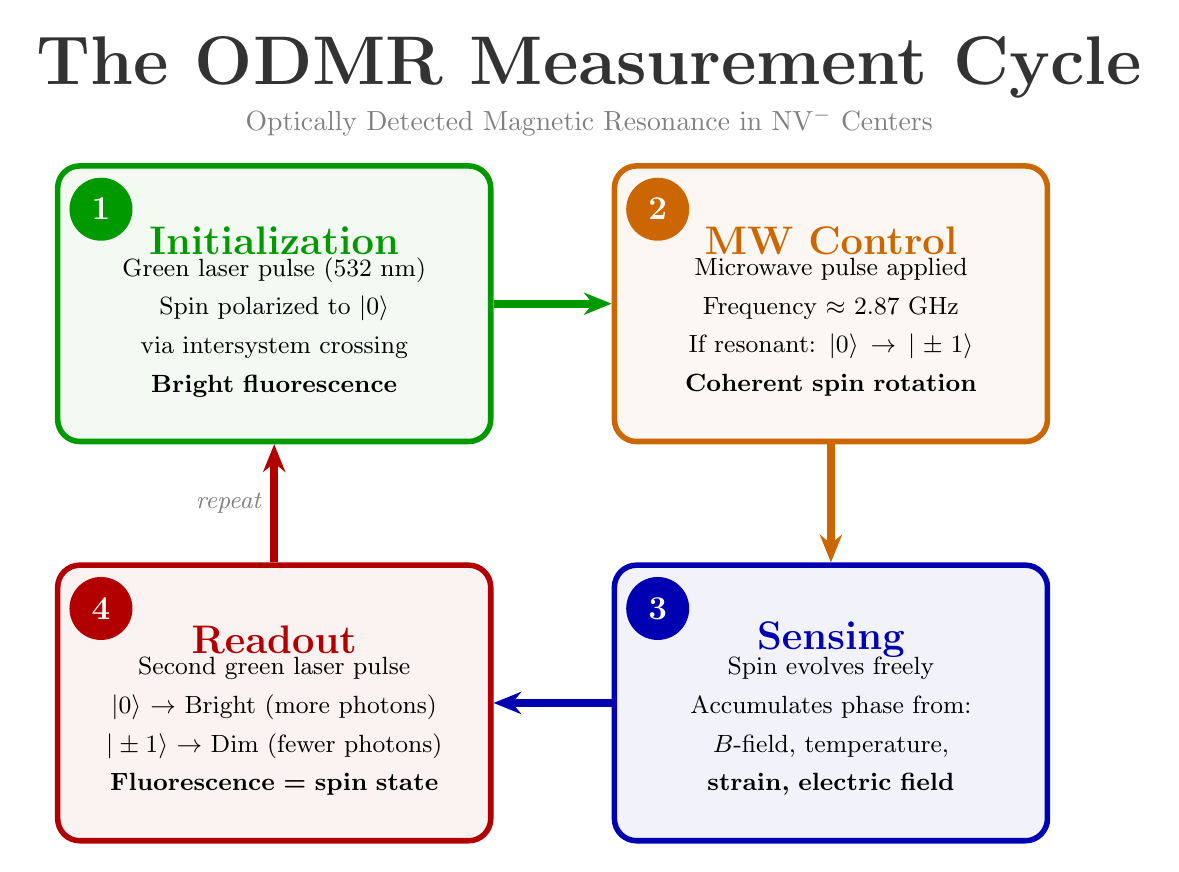
\begin{tikzpicture}[
    stepbox/.style={
        rectangle,
        rounded corners=8pt,
        minimum width=5.5cm,
        minimum height=3.5cm,
        draw=#1,
        line width=2pt,
        fill=#1!5,
        inner sep=10pt,
    },
    steptitle/.style={
        font=\Large\bfseries,
        #1,
    },
    stepdesc/.style={
        font=\small,
        text width=4.5cm,
        align=center,
    },
    stepnum/.style={
        circle,
        fill=#1,
        text=white,
        font=\bfseries\large,
        minimum size=8mm,
        inner sep=0pt,
    },
    arrow/.style={
        -{Stealth[length=10pt, width=8pt]},
        line width=3pt,
        #1,
    },
]

% === Step 1: Initialization ===
\node[stepbox=green!60!black] (init) at (0, 0) {};
\node[stepnum=green!60!black] at ([shift={(-2.2,1.2)}]init.center) {1};
\node[steptitle=green!60!black] at ([shift={(0,0.8)}]init.center) {Initialization};
\node[stepdesc] at ([shift={(0,-0.3)}]init.center) {
    Green laser pulse (532 nm)\\[3pt]
    Spin polarized to $|0\rangle$\\[3pt]
    via intersystem crossing\\[3pt]
    \textbf{Bright fluorescence}
};

% === Step 2: Microwave Control ===
\node[stepbox=orange!80!black, right=1.5cm of init] (ctrl) {};
\node[stepnum=orange!80!black] at ([shift={(-2.2,1.2)}]ctrl.center) {2};
\node[steptitle=orange!80!black] at ([shift={(0,0.8)}]ctrl.center) {MW Control};
\node[stepdesc] at ([shift={(0,-0.3)}]ctrl.center) {
    Microwave pulse applied\\[3pt]
    Frequency $\approx$ 2.87 GHz\\[3pt]
    If resonant: $|0\rangle \rightarrow |\pm1\rangle$\\[3pt]
    \textbf{Coherent spin rotation}
};

% === Step 3: Sensing ===
\node[stepbox=blue!70!black, below=1.5cm of ctrl] (sense) {};
\node[stepnum=blue!70!black] at ([shift={(-2.2,1.2)}]sense.center) {3};
\node[steptitle=blue!70!black] at ([shift={(0,0.8)}]sense.center) {Sensing};
\node[stepdesc] at ([shift={(0,-0.3)}]sense.center) {
    Spin evolves freely\\[3pt]
    Accumulates phase from:\\[3pt]
    $B$-field, temperature,\\[3pt]
    \textbf{strain, electric field}
};

% === Step 4: Readout ===
\node[stepbox=red!70!black, left=1.5cm of sense] (read) {};
\node[stepnum=red!70!black] at ([shift={(-2.2,1.2)}]read.center) {4};
\node[steptitle=red!70!black] at ([shift={(0,0.8)}]read.center) {Readout};
\node[stepdesc] at ([shift={(0,-0.3)}]read.center) {
    Second green laser pulse\\[3pt]
    $|0\rangle \rightarrow$ Bright (more photons)\\[3pt]
    $|\pm1\rangle \rightarrow$ Dim (fewer photons)\\[3pt]
    \textbf{Fluorescence = spin state}
};

% === Arrows ===
\draw[arrow=green!60!black] (init.east) -- (ctrl.west);
\draw[arrow=orange!80!black] (ctrl.south) -- (sense.north);
\draw[arrow=blue!70!black] (sense.west) -- (read.east);
\draw[arrow=red!70!black] (read.north) -- (init.south)
    node[midway, left, font=\small\itshape, text=gray] {repeat};

% === Title ===
\node[font=\Huge\bfseries, text=black!80] at (4, 3) {The ODMR Measurement Cycle};

% === Subtitle ===
\node[font=\normalsize, text=gray] at (4, 2.3) {
    Optically Detected Magnetic Resonance in NV$^-$ Centers
};

\end{tikzpicture}
\end{document}
